%%%%%%%%%%%%%%%%%%%%%%%%%%%%%%%%%%%%%%%%%%%%%%%%%%%%%%%%%%%%%%%%%%%%%%%%%%%%
%%%%%                          GLOSSAIRE                              %%%%%%
%%%%%%%%%%%%%%%%%%%%%%%%%%%%%%%%%%%%%%%%%%%%%%%%%%%%%%%%%%%%%%%%%%%%%%%%%%%%

\phantomsection 
\addcontentsline{toc}{chapter}{Confusing concepts - Disambiguation} \mtcaddchapter
\label{Ann:gloss}
\addtocontents{toc}{\protect\addvspace{10pt}}

\vspace*{-1.6cm}
\begin{flushright}
\section*{\fontsize{20pt}{20pt}\selectfont\textnormal{Confusing concepts - Disambiguation}}
\end{flushright}
\vspace{-0.2cm}


\lhead[\fancyplain{}{Confusing concepts - Disambiguation}]
      {\fancyplain{}{}}
\chead[\fancyplain{}{}]
      {\fancyplain{}{}}
\rhead[\fancyplain{}{}]
      {\fancyplain{}{Confusing concepts - Disambiguation}}
\lfoot[\fancyplain{}{}]
      {\fancyplain{}{}}
\cfoot[\fancyplain{}{\thepage}]
      {\fancyplain{}{\thepage}}
\rfoot[\fancyplain{}{}]%
     {\fancyplain{}{\scriptsize}}

%%%%%%%%%%%%%%%%%%%%%%%%%%%%%%%%%%%%%%%%%%%%%%%%%%%%%%%%%%%%%%%%%%%%%%%%%%
%%%%%                      Start part here                          %%%%%%
%%%%%%%%%%%%%%%%%%%%%%%%%%%%%%%%%%%%%%%%%%%%%%%%%%%%%%%%%%%%%%%%%%%%%%%%%%

\lettrine[lines=1]{S}{ }ome terms used along this thesis may lead to confusion to an uninitiated person, as they are closely related, but describe slightly different concepts. Some others have whole different meanings, depending on the field which employs them. This glossary compares and clarifies them.

\vspace*{0.7cm}

\noindent\underline{Marker vs. Keypoint:}

\textbf{Markers} are objects attached to the body of the user, often small and round. They are used to indirectly track the posture of a user. Markers can sometimes be active and emit light, instead of passive and reflect light. They can also be anchored to the bone, for a more precise analysis exempt from Soft Tissue Artifact (STA). A marker-based analysis commonly refers to the use of passive markers, glued to the skin of the user.

\textbf{Keypoints} are points of interest detected by a machine learning model, either in 2D or in 3D space. They can estimate the location of a human joint, or of a body part, or else of any point of interest of any object. 

Once triangulated, keypoints can be treated as \textbf{virtual markers}, for example while running inverse kinematic (IK) analysis. Calculated markers are another kind of virtual markers, which can for example represent joint centers, or markers which have fallen off the body during capture. \textbf{End-effectors} are the equivalent of markers in the field of robotics.

\vspace*{0.5cm}

\noindent\underline{Markerless vs. Sensorless:}

\textbf{Markerless} systems don't use any markers, but they can use other sensors, such as Inertial Measurement Units (IMUs). 

In contrast, \textbf{sensorless} systems don't involve any wearable markers nor any sensors. This also goes for sensorless dynamic analysis, which does not use any force sensors, or for muscle activation analysis, which does not use any Electromyography (EMG) sensor. 

Note that approaches only using video (RGB), or depth-field video (RGB-D) sensors are usually considered sensorless, as they do not involve any body instrumentation, and thus do not imply any particular alteration to the environment or behavior of the user.

\vspace*{0.5cm}

\noindent\underline{Gold standard vs. Silver standard:}

A \textbf{gold-standard} method refers to the most accurate of the currently available methods, which can be used as a reference to assess the performance of other methods. Bone-anchored pins, Magnetic Resonance Imaging (MRI), biplanar videoradiography, or 3D ultrasounds are usually considered as gold-standard techniques for posture analysis. In contrast, marker-based methods cannot be rigorously considered as such, since they are sensitive to Soft Tissue Artifact (STA) and to positioning variability from the operator. Hence, they are referred to as \textbf{silver-standard} methods. 

However, the previously listed methods are not available for most sports activities, and thus cannot be considered as standards at all. Hence, in this case, marker-based approaches are sometimes referred to as gold-standard, as opposed to IMU or markerless systems, which are then considered as silver-standard.

\vspace*{0.5cm}

\noindent\underline{Silhouette vs. Shape:}

A \textbf{silhouette} is the 2D cutout of a human being on an image. Silhouette segmentation is a specific case of \textbf{object segmentation}. 

A \textbf{shape} is the equivalent of a silhouette in 3D space. A human shape can be used to characterize pose, like 3D keypoints do, but also morphology. A \textbf{mesh} is the geometric representation of a shape, divided into smaller 2D cells (Figure~\ref{fig_meshmodel}).

\begin{figure}[hbtp]
	\centering
            \def\svgwidth{1\columnwidth}
            \fontsize{10pt}{10pt}\selectfont
            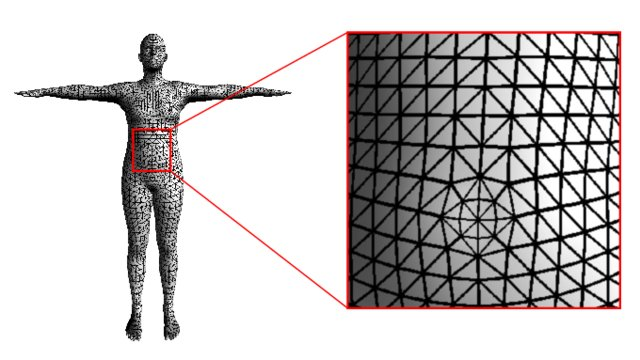
\includegraphics[width=0.6\linewidth]{"../Annexes/Figures/Mesh_model.jpg"}
            \caption{The SMPL mesh model characterizes a 3D human shape. Image from \cite{Wu2020}.}
            \label{fig_meshmodel}
\end{figure}
\FloatBarrier

\vspace*{0.5cm}

\noindent\underline{Machine learning vs. Deep learning:}

Machine learning and Deep Learning, as well as Artificial Intelligence, Artificial Neural Networks, or Convolutional Neural Networks, are sometimes used interchangeably. However, they do not exactly refer to the same concepts (Figure~\ref{fig_ai}).

\textbf{Artificial Intelligence (AI)} concerns the general concept of machines being able to perform tasks that would seem to require human intelligence, or even to sense, reason, and act accordingly. 

\textbf{Machine learning (ML)} is a subset of AI, and refers to the concept of machines being able to learn and improve as they are exposed to data. It is a data-driven approach, as opposed to knowledge-driven ones.\\
\textbf{Artificial Neural Networks (ANN)} are a specific way of performing ML, by using a network of units inspired from the natural neuron, and thus mimicking the brain. 

\textbf{Deep Learning (DL)} refers to an ANN with more than 3 layers of neurons.

\textbf{Convolutional Neural Networks (CNN)} are a type of ANN which is particularly suited for image processing.

\begin{figure}[hbtp]
	\centering
            \def\svgwidth{1\columnwidth}
            \fontsize{10pt}{10pt}\selectfont
            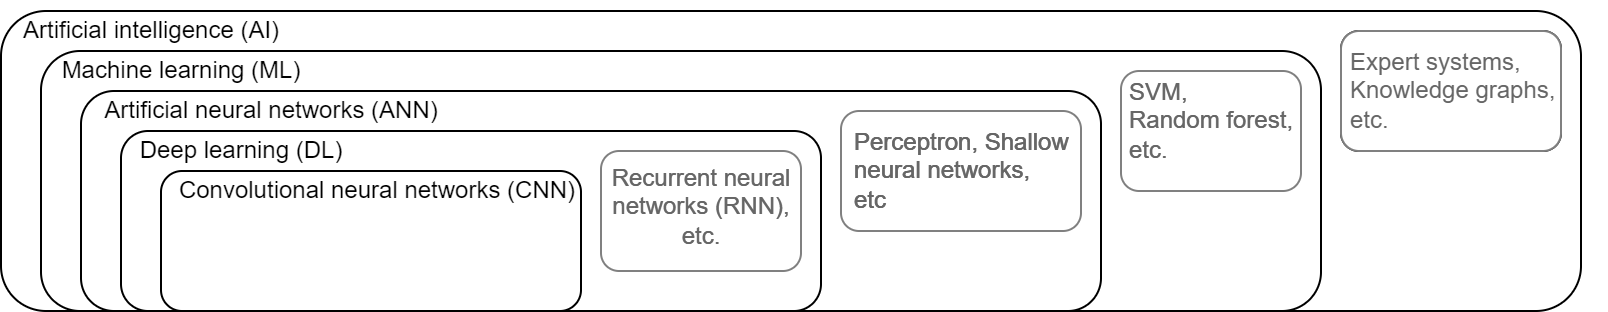
\includegraphics[width=\linewidth]{"../Annexes/Figures/AI_CNN_etc.png"}
            \caption{Inclusion diagram for the concepts of Artificial intelligence, Machine learning, Artificial neural networks, Deep learning, and Convolutional neural networks.}
            \label{fig_ai}
\end{figure}
\FloatBarrier
\vspace*{0.5cm}

\noindent\underline{Dataset vs. Labels: }

A \textbf{dataset} is a collection of data used to train a machine learning model. These data need to be labelled prior to training. \textbf{Labels} and \textbf{annotations} can generally be considered as synonyms. Certain datasets come with several kinds of annotations: keypoints, instance segmentation, or image classification for example. Note that a same dataset can be annotated with several keypoint instances, e.g., one focusing on hands, and the other one on the full body.

Once labeled, a dataset can be fed to a deep learning \textbf{architecture}, or \textbf{algorithm}, upon which is appended a \textbf{feature extractor}, or \textbf{backbone}, specific to the chosen labelling convention. A \textbf{model} results from this training, which can then be used to predict the labels of new data. Hand-labeled dataset can be used as \textbf{benchmarks} for assessing the model accuracy or speed. 

In the everyday use, datasets, labeling or annotation, architecture, and models, tend to be used in a confusing way. For instance, the standard OpenPose model has been trained on the COCO and MPII dataset, annotated with COCO, MPII, and additional foot keypoints, on the OpenPose architecture. This results in the OpenPose body\_25 model. 

\vspace*{0.5cm}

\noindent\underline{Single-view vs. Multi-view:}

A \textbf{multi-view} (or multiview) system uses several cameras, while a \textbf{single-view}, or \textbf{monocular} one, uses only one. While multi-view systems are always used to infer 3D information, monocular ones can either focus on 2D or 3D information retrieval.

\textbf{Single-image}, or \textbf{single-frame} approaches, specifically analyze one single image from a single view. In practice, video approaches often perform their analysis image by image.

\vspace*{0.5cm}

\noindent\underline{Kinematics vs. Kinetics: }

\textbf{Kinematics} describes the motion of points (e.g., heel marker), bodies (e.g., foot segment), or systems of bodies (e.g., human whole body). This can involve studying positions or angles, as well as linear and angular velocities or accelerations. However, kinematics studies motion only in a geometric way, without considering its causes. It deals with the \emph{equations of motion}.

On the other hand, \textbf{kinetics} deals with the causes of motion. According to Newton's second law of motion, the forces that induce the motion of a body are obtained by multiplying its acceleration by its mass. Hence, unlike kinematics, kinetics takes masses into account (or more generally, inertial properties). It involves considering external forces (e.g., gravity or ground reaction forces), internal forces (e.g., joint moments or individual muscle forces), or energy or power (e.g., kinetic energy). More generally, kinetics deals with the \emph{laws of motion}.

\textbf{Dynamics} includes both kinematics and kinetics. However, note that in practice, kinetics and dynamics are often used as synonyms. \textbf{Statics} is a special case of dynamics where the sum of forces is zero, and consequently, so is the acceleration. Thus, either the velocity of the object is constant, or it is not moving at all. 

\vspace*{0.5cm}

\noindent\underline{Spatio-temporal parameters vs Joint kinematics:}

\textbf{Spatio-temporal parameters} are handcrafted indicators used for the kinematic analysis of a specific task. Among other, they can include step length or cadence for gait analysis, or the reach of the jab or the excursion of the center of motion for boxing analysis.

\textbf{Joint kinematics} is the study of joint motion, such as joint angle or joint laxity, or joint velocities and accelerations.

Technically, both spatio-temporal parameters and joint kinematics fall under the umbrella of kinematic data; however, in the customary usage, kinematics describes joint kinematics.


\vspace*{0.5cm}
\noindent\underline{Forward kinematics vs. Inverse kinematics} (and global vs. local optimization):

In the multi-body analysis of human motion, \textbf{forward kinematics generally involves finding the positions of M markers $\overrightarrow{X}$ from N joint angles $\overrightarrow{q}$}. Markers are more formally called end-targets, and joint angles degrees of freedom. In other words, forward kinematics aims to solve the equation $\overrightarrow{X}=f(\overrightarrow{q})$. Marker positions can usually be solved analytically, with a combination of trigonometric formulas. However, this assumes that segment dimensions and marker placement on each segment are known, and that soft tissue artifacts and measurement inaccuracies can be neglected.

Conversely, \textbf{inverse kinematics deals with finding joint angles from marker positions}, and thus with solving the equation $\overrightarrow{q}=f^{-1}(\overrightarrow{X})$. Instead of prescribing the movement joint by joint, the idea is to provide one or several known marker positions, that will be reached with unknown joint angles. However, in practice $f$ is not generally invertible, and there is either an infinite amount of ways to reach targets, or none at all targets are out of reach. Consequently, optimization methods need to be leveraged. Inverse kinematics involves defining a kinematic chain, with segment dimensions and joint properties. It is sometimes called \emph{Multi-body Kinematic Optimization} (MKO), or \emph{Global Optimization} (GO). Note that this latter term should not be favored, since these methods do not pretend to look for a global minimum. They are only global in the sense that they consider all joints at once.

Another approach for finding joint angles is the \textbf{6DoF (6 Degrees of Freedom)} one, sometimes called \emph{Single-body Kinematic Optimization} (SKO). The idea is to compute each segment position and orientation independently, and then deduces inter-segmental angles. It does not assume any prior knowledge on segment dimensions nor joint properties, but it involves having at least 3 markers per segment.

\textbf{Direct kinematics} is usually considered to be a synonym of forward kinematics. However, when there are exactly as many joint angles as marker coordinates, both of them can be equally solved. Hence, the term direct kinematics is sometimes also employed to describe the analytical calculation of M joint angles from the position of M markers.





% There is an exact solution, which can be calculated . Unlike in robotics, joint angles are hardly directly measurable in human motion analysis, which makes forward kinematics of little interest in this field.\\

% either more segment coordinates than unknown degrees of freedom (the system is overdetermined), or less (it is underterermined).

% segment poses are usually not all known, and there are then more unknown joint degrees of freedom than known segment poses: the system is underdetermined. This implies that the target can be reached with different joint configurations. Consequently, no exact solution can be found, and one needs to turn to numerical methods in order to find an "optimal" solution.\\

% \vspace*{0.5cm}

% \noindent\underline{Linear vs. Non-linear system, Overdetermined/overconstrained vs. Underdetermined/redundant system, \\Direct vs.Numerical solution:}\\


% x=f(q), need to find f-1(x)=q. However, f not necessarily invertible. x= M marker position (measurements), q= N joint angles (unknown degrees of freedom)

% if linear <-> AX=B: 
%       if M=N, A is square and invertible -> exact solution (assuming $rank(A)=M$, i.e., that none of the lines can be expressed as a linear combination of the others)
%       . Direct / analytical / symbolic / explicit method
%       Ex: 3D joint angles with 3 markers per segment

%       if M>N, A is overdetermined -> no exact solution, but exists one closed-form solution 
%       . Direct / algebraic / analytical / symbolic method, eg given with the Moore-Penrose pseudo-inverse -> SVD  
%       Ex: Single-body kinematic optimization, calibration with one single image of a checkerboard, linear-eigen triangulation, single-body kinematic optimization
%       . Or iterative methods

%       if M<N, A is underdetermined -> infinite amount of solutions approximate
%       . Iterative / numerical method? start with initial guess
%       Ex: calib with several checkerboard images when no disto

% if non linear (squares, cos, derivatives), over or underdetermined:
%       . Iterative / numerical method, start with initial guess
%       ex: calib when taking distortion into account, with several checkerboard images, or with a wand, 
%       multi-body kinematic optimization


% Où mettre ça :
%       Optimization: direct or iterative method?
%       Linear/non-linear least-squares ?
%       Inverse kinematics non linear (cos) ?
      



% \vspace*{0.5cm}
% \noindent\underline{Overdetermined vs. Underdetermiend system:}\\

% However, in practice there are usually less known marker coordinates than unknown joint degrees of freedom, and $f$ is not invertible: the system is underdetermined, and there is an infinite amount of solutions (or none at all). 

% is either an infinite amount of solutions (if M<N, there are fewer markers than degrees of freedom, and the system is underdetermined), or none at all (if M>N, the system is overdetermined).


% f(X) = Q
% A system of M linear equations can be written as $\textbf{A} \overrightarrow{X}=\overrightarrow{B}$. $\overrightarrow{X}$ contains the N degrees of freedom to be determined, which can represent N unknown joint angles for example. $\overrightarrow{B}$ contains M observations, marker coordinates for example. \textbf{A} is a matrix of size $M \times N$, each of the M lines expressing the values each joint angle has taken to lead to the observed marker position. We assume that none of the lines can be expressed as a linear combination of the others: $rank(A)=M$.

% - If M = N, there are as many observations as degrees of freedom, e.g., as many markers coordinates as unknown joint angles. Then, an exact solution can be calculated analytically/symbolically. This is for example the case for single-body direct kinematics.

% - If more markers than degrees of freedom (M>N): rang syst > nb equations. overdetermined, no solution. (calibration with more coordinates of 2D-3D correspondences than unknown calibration parameters, triangulation from more than 2 cameras, single and multi body optimized kinematics with more than 3 markers per segment)
% Find \emph{approximate / optimal} solution, on minimise objective/loss function ||f(X)-B||2 :
% 1. Calcul direct quasi analytique (calcul svd itératif) (closed form) si connues = linear combinaison d'inconnues: f(x)-q peut s'ecrire AX - B. 
% Pseudo solution = linear least square solution, via SVD
% (calib sans disto, )
% 2. Sinon, Calcul numérique iteratif from initial guess
% Non linear least square solution, eg via Levenberg-Marquardt: linearisation via développement Taylor 1er ordre pour passer par la Jacobienne, pseudo inverse, on retombe sur SVD
% (note: peut aussi etre utilisé avec systemes linéaires, plus rapide si beaucoup de var, typiquement 1,000,000. Pas pour nous)

% - If less markers than degrees of freedom (M<N): rang syst < nb equations. underdetermined, infinite solutions
% (multi body optimized kinematics with less markers than unknown joint parameters): 
% 1. damped least-square // pseudo-inverse jacobian // levenberg Marquardt, choose sol closest to previous position (initial guess)
% 2. Ou global optim, ou kalman smoother, etc



% voire heuristique (par à la découverte au hasard pour éviter minimums locaux plutôt que convergence rigoureuse) 
% voire learning






% Closed Chain :
% https://sci-hub.se/https://link.springer.com/article/10.1007/s11044-013-9366-7





\vspace*{0.5cm}
\noindent\underline{Generalized coordinates vs. Cartesian coordinates:}

In the field of biomechanics, \textbf{generalized coordinates} are an extension of \textbf{Cartesian coordinates}, used to describe joint configurations, whether they be linear or angular. Similarly, generalized velocities can be angular velocities, generalized forces moments, etc. \textbf{Plücker coordinates} are sometimes used to consider both sets of coordinates in a single 6D system (3D positions + 3D orientations).


% Joints vs. Constraints: 
% hard (joint dof restrictions, of coupling equations between dof) and soft (penalties in the objective function) \cite{Begon2018}
% https://simtk.org/plugins/phpBB/viewtopicPhpbb.php?f=91&t=15244&p=44312&start=0&view=

% top-down vs. bottom-up vs. single-person: 

% CONSTRAINED
% dof
% soft, hard 
% joint limits, closed chain